% Pipeline block diagram: input -> preprocess -> masks / measure -> filter -> output -> compare.
% Build: lualatex pipeline_block_diagram.tex
% File: pipeline_block_diagram.tex · Git: Michael G. Prisant 4c7b2f1 · Txd: 11/12/26 with local modifications!
\documentclass[border=6pt]{standalone}
\usepackage{libertinus}
\usepackage{tikz}
\usetikzlibrary{positioning,arrows.meta,fit,backgrounds,calc}

\definecolor{ink}{HTML}{1F2933}
\definecolor{inbg}{HTML}{E8EEF5}
\definecolor{stagebg}{HTML}{FFFFFF}
\definecolor{rulebg}{HTML}{FBF6E9}
\definecolor{refbg}{HTML}{EAF3EA}
\definecolor{rim}{HTML}{52606D}

\begin{document}
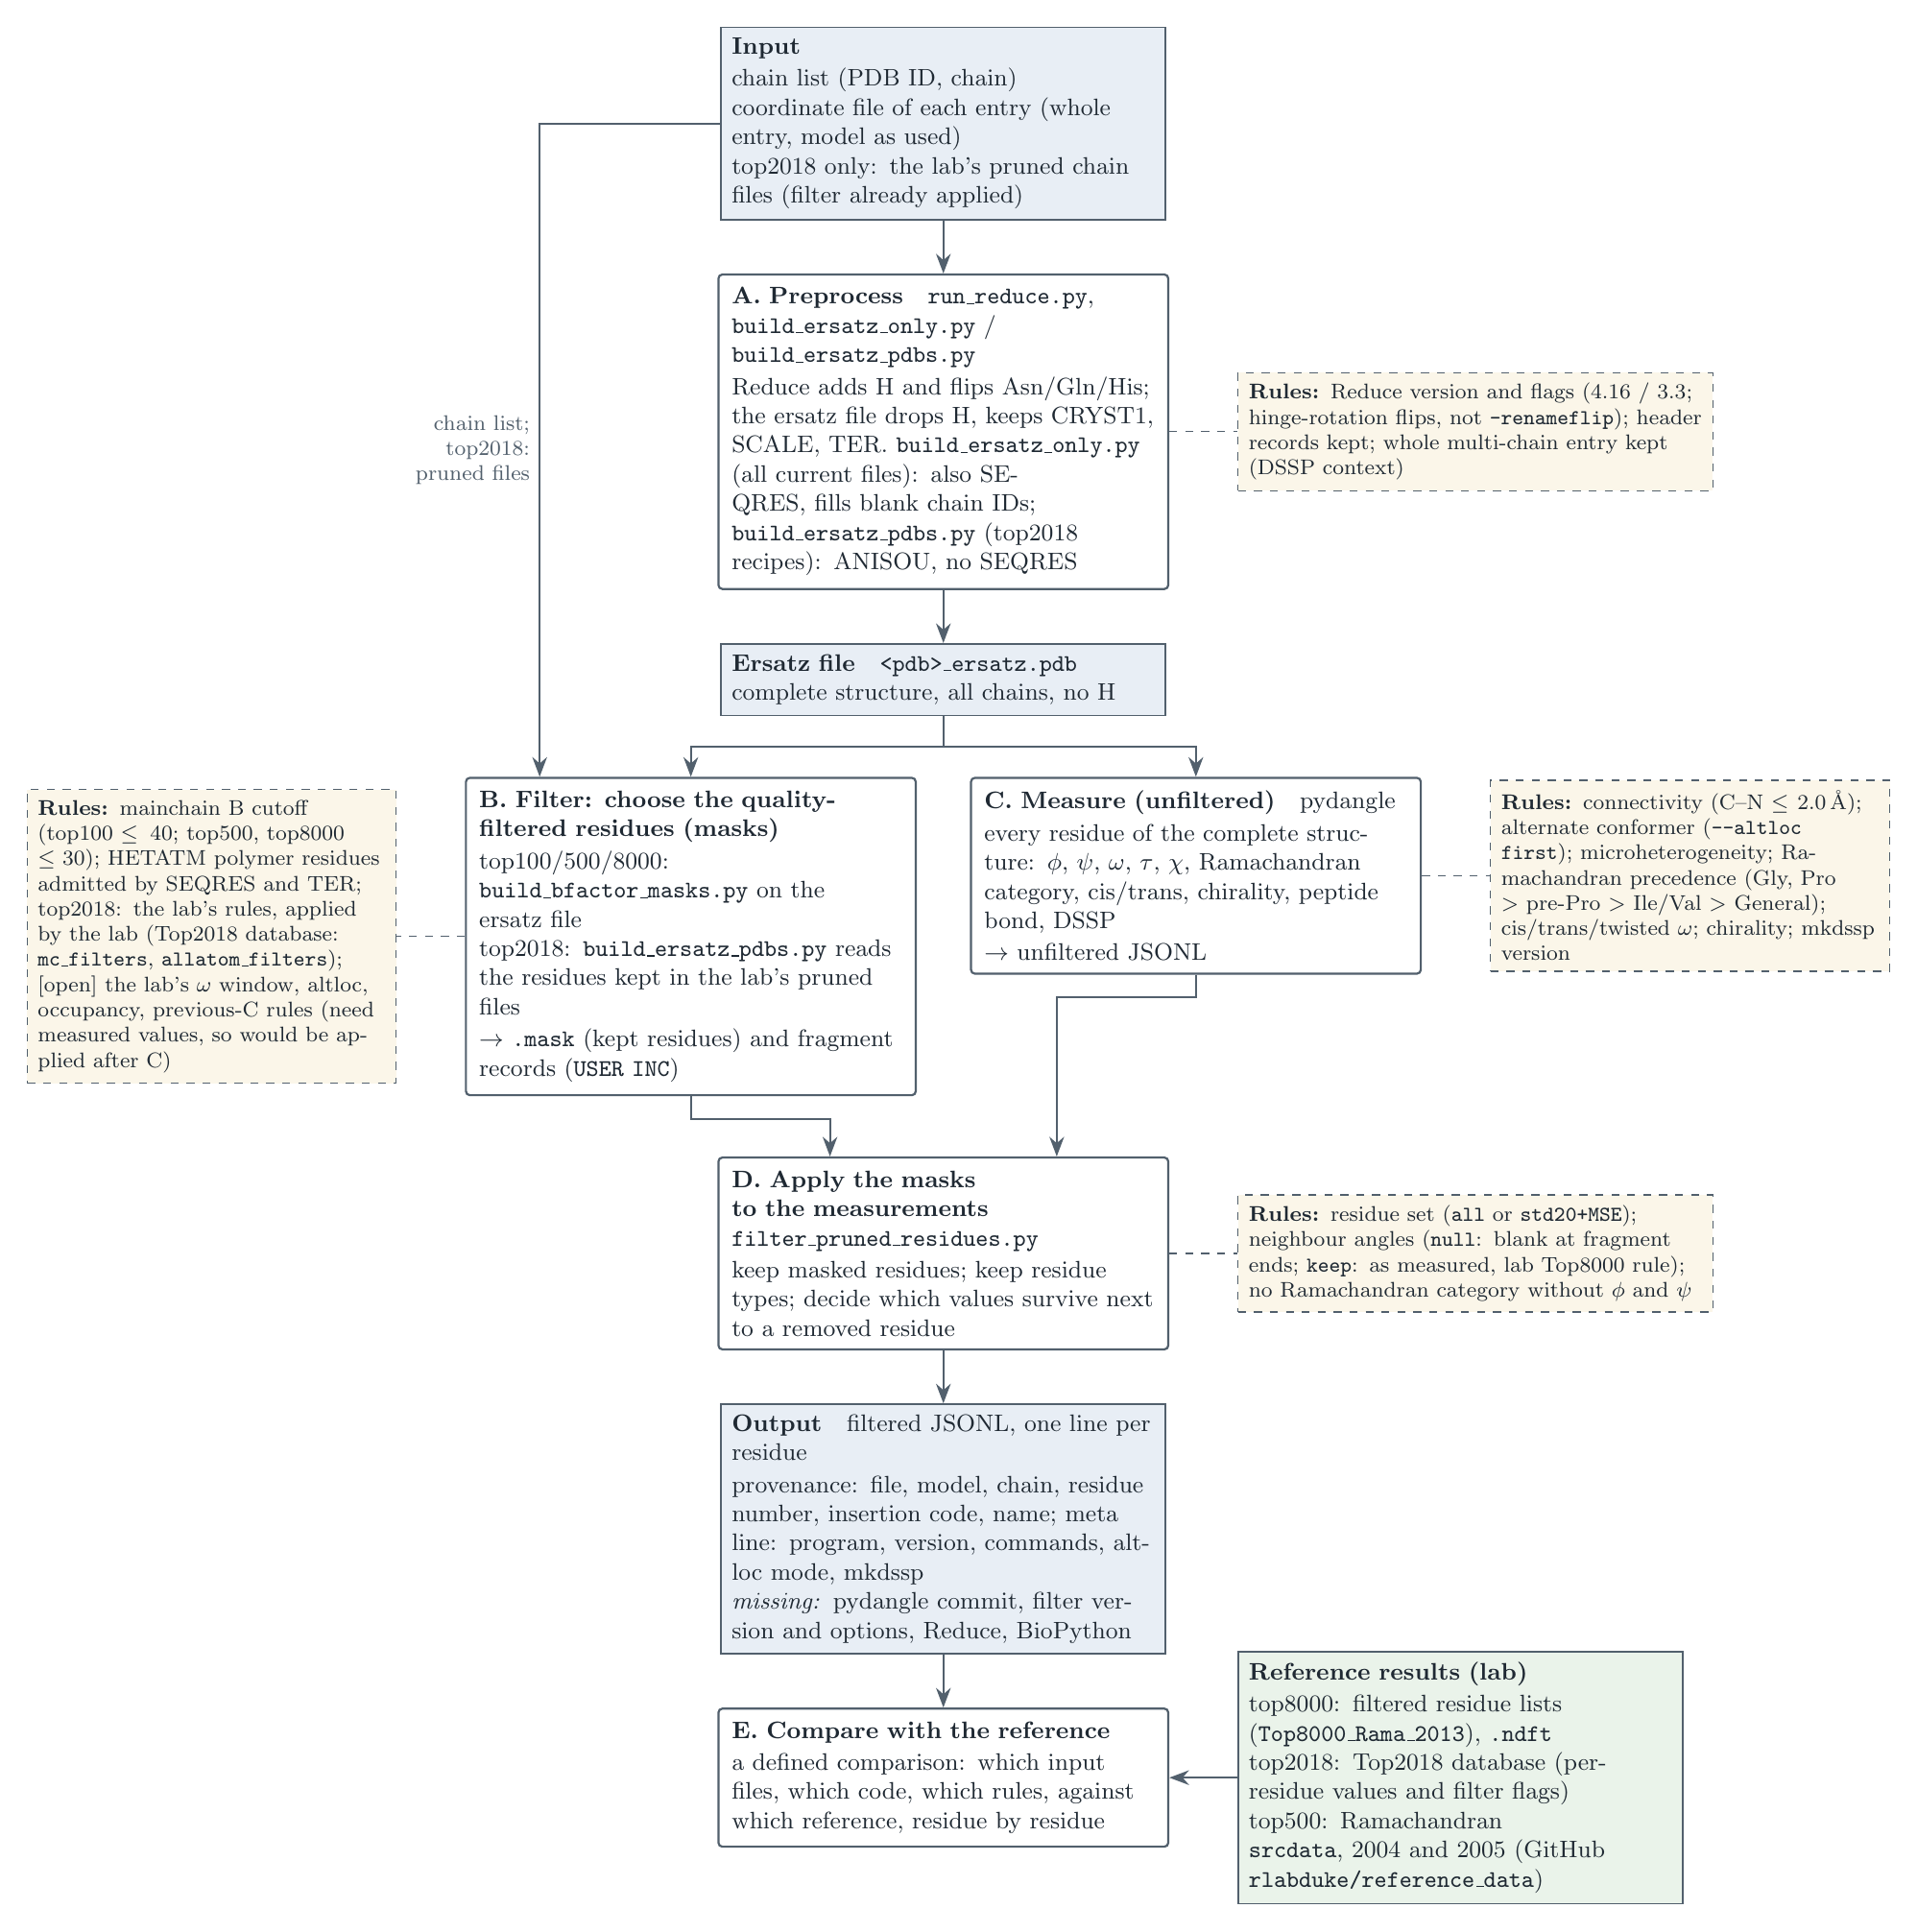
\begin{tikzpicture}[
  font=\small, color=ink,
  node distance=7mm and 9mm,
  >={Stealth[length=2.6mm]},
  flow/.style={->, line width=0.7pt, rim},
  stage/.style={draw=rim, line width=0.8pt, fill=stagebg, rounded corners=1.5pt,
                text width=56mm, align=left, inner sep=5pt},
  data/.style={draw=rim, line width=0.6pt, fill=inbg, text width=56mm,
               align=left, inner sep=4pt},
  rules/.style={draw=rim, line width=0.5pt, dashed, fill=rulebg, text width=60mm,
                align=left, inner sep=4pt, font=\footnotesize},
  ref/.style={draw=rim, line width=0.6pt, fill=refbg, text width=56mm,
              align=left, inner sep=4pt},
  title/.style={font=\bfseries\small},
]

% ---------- inputs ----------
\node[data] (in) {\textbf{Input}\\[1pt]
  chain list (PDB ID, chain)\\
  coordinate file of each entry (whole entry, model as used)\\
  top2018 only: the lab's pruned chain files (filter already applied)};

% ---------- stage A ----------
\node[stage, below=of in] (pre) {\textbf{A. Preprocess}\quad
  \texttt{run\_reduce.py}, \texttt{build\_ersatz\_only.py} / \texttt{build\_ersatz\_pdbs.py}\\[1pt]
  Reduce adds H and flips Asn/Gln/His; the ersatz file drops H, keeps
  CRYST1, SCALE, TER. \texttt{build\_ersatz\_only.py} (all current files): also SEQRES,
  fills blank chain IDs; \texttt{build\_ersatz\_pdbs.py} (top2018 recipes): ANISOU, no SEQRES};
\node[rules, right=of pre] (preR) {\textbf{Rules:} Reduce version and flags
  (4.16 / 3.3; hinge-rotation flips, not \texttt{-renameflip});
  header records kept; whole multi-chain entry kept (DSSP context)};

\node[data, below=of pre] (ers) {\textbf{Ersatz file}\quad \texttt{<pdb>\_ersatz.pdb}\\
  complete structure, all chains, no H};

% ---------- stages B and C side by side below ersatz ----------
\node[stage, below left=8mm and -26mm of ers] (mask) {\textbf{B. Filter: choose the quality-filtered residues (masks)}\\[1pt]
  top100/500/8000: \texttt{build\_bfactor\_masks.py} on the ersatz file\\
  top2018: \texttt{build\_ersatz\_pdbs.py} reads the residues kept in the
  lab's pruned files\\[1pt]
  $\to$ \texttt{.mask} (kept residues) and fragment records (\texttt{USER INC})};
\node[stage, below right=8mm and -26mm of ers] (meas) {\textbf{C. Measure (unfiltered)}\quad pydangle\\[1pt]
  every residue of the complete structure:
  $\phi$, $\psi$, $\omega$, $\tau$, $\chi$, Ramachandran category,
  cis/trans, chirality, peptide bond, DSSP\\[1pt]
  $\to$ unfiltered JSONL};

\node[rules, left=of mask, text width=46mm] (maskR) {\textbf{Rules:} mainchain B cutoff
  (top100 $\le 40$; top500, top8000 $\le 30$);
  HETATM polymer residues admitted by SEQRES and TER;
  top2018: the lab's rules, applied by the lab
  (Top2018 database: \texttt{mc\_filters}, \texttt{allatom\_filters});
  [open] the lab's $\omega$ window, altloc, occupancy, previous-C rules
  (need measured values, so would be applied after C)};
\node[rules, right=of meas, text width=50mm] (measR) {\textbf{Rules:} connectivity (C--N $\le 2.0$\,\AA);
  alternate conformer (\texttt{--altloc first}); microheterogeneity;
  Ramachandran precedence (Gly, Pro $>$ pre-Pro $>$ Ile/Val $>$ General);
  cis/trans/twisted $\omega$; chirality; mkdssp version};

% ---------- stage D ----------
\coordinate (mid) at ($(mask.south)!0.5!(meas.south)$);
\node[stage, below=16mm of mid] (filt) {\textbf{D. Apply the masks to the measurements}\quad
  \texttt{filter\_pruned\_residues.py}\\[1pt]
  keep masked residues; keep residue types; decide which values
  survive next to a removed residue};
\node[rules, right=of filt] (filtR) {\textbf{Rules:} residue set (\texttt{all} or
  \texttt{std20+MSE}); neighbour angles (\texttt{null}: blank at fragment ends;
  \texttt{keep}: as measured, lab Top8000 rule); no Ramachandran category
  without $\phi$ and $\psi$};

% ---------- output ----------
\node[data, below=of filt] (out) {\textbf{Output}\quad filtered JSONL, one line per residue\\[1pt]
  provenance: file, model, chain, residue number, insertion code, name;
  meta line: program, version, commands, altloc mode, mkdssp\\
  \emph{missing:} pydangle commit, filter version and options, Reduce,
  BioPython};

% ---------- stage E ----------
\node[stage, below=of out] (cmp) {\textbf{E. Compare with the reference}\\[1pt]
  a defined comparison: which input files, which code, which rules,
  against which reference, residue by residue};
\node[ref, right=of cmp] (refs) {\textbf{Reference results (lab)}\\[1pt]
  top8000: filtered residue lists (\texttt{Top8000\_Rama\_2013}), \texttt{.ndft}\\
  top2018: Top2018 database (per-residue values and filter flags)\\
  top500: Ramachandran \texttt{srcdata}, 2004 and 2005 (GitHub \texttt{rlabduke/reference\_data})};

% ---------- arrows ----------
\draw[flow] (in) -- (pre);
\draw[flow] (pre) -- (ers);
\draw[flow] (ers.south) -- ++(0,-4mm) -| (mask.north);
\draw[flow] (ers.south) -- ++(0,-4mm) -| (meas.north);
\draw[flow] (in.west) -| ([xshift=-20mm]mask.north)
  node[pos=0.75, left, font=\footnotesize, align=right]{chain list;\\ top2018:\\ pruned files};
\draw[flow] (mask.south) -- ++(0,-3mm) -| ([xshift=-15mm]filt.north);
\draw[flow] (meas.south) -- ++(0,-3mm) -| ([xshift=15mm]filt.north);
\draw[flow] (filt) -- (out);
\draw[flow] (out) -- (cmp);
\draw[flow] (refs) -- (cmp);

\draw[dashed, rim, line width=0.4pt] (pre) -- (preR);
\draw[dashed, rim, line width=0.4pt] (mask) -- (maskR);
\draw[dashed, rim, line width=0.4pt] (meas) -- (measR);
\draw[dashed, rim, line width=0.4pt] (filt) -- (filtR);

\end{tikzpicture}
\end{document}
